\documentclass[journal,12pt,twocolumn]{IEEEtran}
\usepackage[cmex10]{amsmath}
\usepackage{graphicx}
\usepackage{pgfplots}
\usepackage[font=normal]{caption}
\pgfplotsset{compat=newest}
\pgfplotsset{scaled y ticks=false}
\usepgfplotslibrary{groupplots}
\usepgfplotslibrary{dateplot}

\usepackage{tikz}

\pgfplotsset{compat=1.11,
 /pgfplots/ybar legend/.style={
 /pgfplots/legend image code/.code={
 \draw[##1,/tikz/.cd,yshift=-0.25em]
 (0cm,0cm) rectangle (3pt,0.8em);},
 },
}
\let\vec\mathbf
\newcommand{\myvec}[1]{\ensuremath{\begin{pmatrix}#1\end{pmatrix}}}
\providecommand{\brak}[1]{\ensuremath{\left(#1\right)}}
\newcommand\numberthis{\addtocounter{equation}{1}\tag{\theequation}}

\title{Lines using Python}
\author{Ahilan R - FWC22090}
\date{\today}

\begin{document}
\maketitle

\subsection*{\textbf{Problem}}
The equations to the pair of opposite sides of a parallelogram are 
\begin{align}
		x^2-5x+6 &= 0	\text{,}	\label{eq:lp1} \\
		y^2-6y+5 &= 0	\text{.}\label{eq:lp2}
\end{align} 
Find the equations to the diagonals of the parallelogram.

\subsection*{\textbf{Solution}}

%\subsection{$x$ and $y$ Intercepts}

%On comparing \eqref{eq:lp1} and \eqref{eq:lp2} to  
%\begin{align*}
%		a_1x^2+b_1x+c_1&=0	 \text{,}\\
%		a_2y^2+b_2y+c_2&=0	\text{.}
%\end{align*}
%we get,
%\begin{align*}
%		a_1&=1 , \quad b_1=-5 , \quad c_1=6 \text{,}\\
%		a_2&=1 , \quad b_2=-6 , \quad c_2=5\text{.}
%\end{align*}
%
%Using quadratic formula, the $x$ and $y$ intercepts of the given lines are 

On factorizing \eqref{eq:lp1} and \eqref{eq:lp2} we get, 
\begin{align*}
	(x-2)(x-3)=0, \\
	(y-1)(y-5)=0.
\end{align*}
So the $x$ and $y$ intercepts of the given lines are 
\medskip
\begin{align*}
	\vec{X_1} &= \myvec{2\\0}, \quad 	\vec{X_2} = \myvec{3\\0}, \\
	\text{ and } \vec{Y_1} &= \myvec{0\\1}, \quad	\vec{Y_2} = \myvec{0\\5}
\end{align*}

%\begin{align*}
%		\vec{X_1} &= \myvec{\cfrac{-b_1 - \sqrt{b_1^2-4a_1c_1}}{2a_1}\\0} \text{,}\\
%		\vec{X_2} &= \myvec{\cfrac{-b_1 + \sqrt{b_1^2-4a_1c_1}}{2a_1}\\0} \text{,}\\
%		\vec{Y_1} &= \myvec{0\\ \cfrac{-b_2 - \sqrt{b_2^2-4a_2c_2}}{2a_2}}\text{,}\\
%		\vec{Y_2} &= \myvec{0\\ \cfrac{-b_2 + \sqrt{b_2^2-4a_2c_2}}{2a_2}}\text{.}
%\end{align*}

%\subsection{Observation}
The pair of straight lines represented by \eqref{eq:lp1} are parallel to y-axis and the pair of straight lines represented by \eqref{eq:lp2} are parallel to x-axis.

%\medskip
%since \eqref{eq:lp1} and \eqref{eq:lp2} are quadratic in single variable.

We can also say that the lines in \eqref{eq:lp1} are normal to $\vec{e_1}$ and the lines in \eqref{eq:lp2} are normal to $\vec{e_2}$,  
where, $\vec{e_1}$ and $\vec{e_2}$ are standard basis vectors, given by
\begin{align*}
		\vec{e_1} = \myvec{1\\0} &\text{ and   }
		\vec{e_2} = \myvec{0\\1} \text{.} 
\end{align*}

%\subsection{Line Equations in Vector Form}
Equations of the sides of parallelogram in vector form,  
\begin{align}
		L_1 &\colon \quad \vec{e_1^{\top}}\brak{{\vec{x}-\vec{X_1}}} = 0\text{,} \label{eq:line_1}\\
		L_2 &\colon \quad \vec{e_2^{\top}}\brak{{\vec{x}-\vec{Y_1}}} = 0\text{,} \label{eq:line_2}\\
		L_3 &\colon \quad \vec{e_1^{\top}}\brak{{\vec{x}-\vec{X_2}}} = 0\text{,} \label{eq:line_3}\\
		L_3 &\colon \quad \vec{e_2^{\top}}\brak{{\vec{x}-\vec{Y_2}}} = 0\text{.} \label{eq:line_4}
\end{align}
%where, $\vec{e_1}$ and $\vec{e_2}$ are standard basis vectors, given by
%\begin{align*}
%		\vec{e_1} = \myvec{1\\0} &\text{ and   }
%		\vec{e_2} = \myvec{0\\1} \text{.} 
%\end{align*}

%\subsection{Obtaining Vertices}
Intersection of given sides yields the vertices of parallelogram. Let's find the point A, say, which is intersection of line $L_1$  and line $L_2$ .\\ %\eqref{eq:line_2} \eqref{eq:line_1}

%\subsection{Diagram}
%\begin{figure}[h]
%\centering
%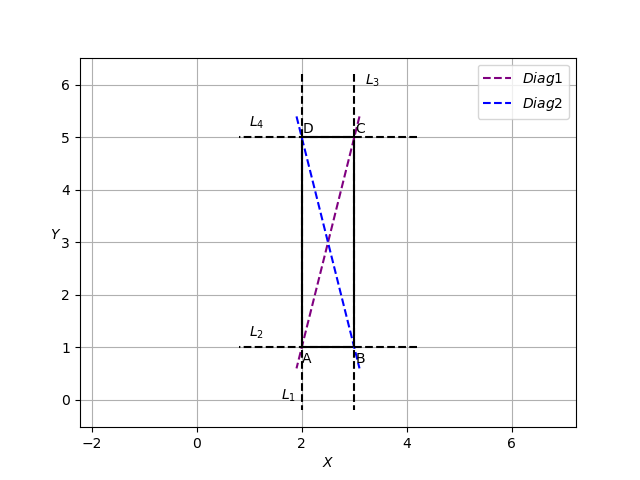
\includegraphics[width=\columnwidth]{figs/plot.png}
%\caption{Parallelogram generated using python}
%\label{fig:rect_py}
%\end{figure}

%\vspace{-0.5cm}

On combining \eqref{eq:line_1} and \eqref{eq:line_2}, 
\begin{align*}
		\myvec{ \vec{e_1} & \vec{e_2}}^{\top}\vec{A}&= \myvec{\vec{e_1}^{\top}\vec{X_1}\\ \vec{e_2}^{\top}\vec{Y_1} }  \\[0.7ex]
		\text{Take,	} \vec{n} &= \myvec{ \vec{e_1} & \vec{e_2}}^{\top} \numberthis \label{eq:n_matrix} \\[0.7ex]
		\implies \vec{A} &= \vec{n}^{-1} \myvec{\vec{e_1}^{\top}\vec{X_1}\\ \vec{e_2}^{\top}\vec{Y_1} }
\end{align*}

%Similarly, the intersection of $L_2$ \eqref{eq:line_2} and $L_3$ \eqref{eq:line_3} 
%\begin{align*}
%	\vec{B} &= \vec{n}^{-1} \myvec{\vec{e_1}^{\top}\vec{X_2}\\ \vec{e_2}^{\top}\vec{Y_1} }
%\end{align*}

Similarly, we can obtain other vertices as
\begin{align*}
	\vec{B} &= \vec{n}^{-1} \myvec{\vec{e_1}^{\top}\vec{X_2}\\ \vec{e_2}^{\top}\vec{Y_1} } \text{, } \\[0.7ex]
	\vec{C} &= \vec{n}^{-1} \myvec{\vec{e_1}^{\top}\vec{X_1}\\ \vec{e_2}^{\top}\vec{Y_2} } \text{,}\\[0.7ex]
		\text{and  }		\vec{D} &= \vec{n}^{-1} \myvec{\vec{e_1}^{\top}\vec{X_2}\\ \vec{e_2}^{\top}\vec{Y_2} } \text{.}
\end{align*}
where,
\begin{align*}
	B & \text{ is the intersection of lines } L_2 \text{ and } L_3, \\[-0.5ex]
	C & \text{ is the intersection of lines } L_3 \text{ and }L_4,\\[-0.5ex]
	D & \text{ is the intersection of lines } L_4 \text{ and }L_1.
\end{align*}

\begin{figure}[h]
\centering
\def\figwidth{\linewidth}
\def\figheight{0.25\textheight} % Feel free to change
% This file was created with tikzplotlib v0.10.1.
\begin{tikzpicture}

\definecolor{darkgray176}{RGB}{176,176,176}
\definecolor{lightgray204}{RGB}{204,204,204}
\definecolor{purple}{RGB}{128,0,128}

\begin{axis}[
height=\figheight,
legend cell align={left},
legend style={fill opacity=0.8, draw opacity=1, text opacity=1, draw=lightgray204},
tick align=outside,
tick pos=left,
width=\figwidth,
x grid style={darkgray176},
xlabel={\(\displaystyle X\)},
xmajorgrids,
xmin=-2.22380952380953, xmax=7.22380952380953,
xtick style={color=black},
y grid style={darkgray176},
ylabel style={rotate=-90.0},
ylabel={\(\displaystyle Y\)},
ymajorgrids,
ymin=-0.52, ymax=6.52,
ytick style={color=black}
]
\addplot [semithick, black, forget plot]
table {%
2 1
2.11111111111111 1
2.22222222222222 1
2.33333333333333 1
2.44444444444444 1
2.55555555555556 1
2.66666666666667 1
2.77777777777778 1
2.88888888888889 1
3 1
};
\addplot [semithick, black, forget plot]
table {%
3 1
3 1.44444444444444
3 1.88888888888889
3 2.33333333333333
3 2.77777777777778
3 3.22222222222222
3 3.66666666666667
3 4.11111111111111
3 4.55555555555556
3 5
};
\addplot [semithick, black, forget plot]
table {%
3 5
2.88888888888889 5
2.77777777777778 5
2.66666666666667 5
2.55555555555556 5
2.44444444444444 5
2.33333333333333 5
2.22222222222222 5
2.11111111111111 5
2 5
};
\addplot [semithick, black, forget plot]
table {%
2 5
2 4.55555555555556
2 4.11111111111111
2 3.66666666666667
2 3.22222222222222
2 2.77777777777778
2 2.33333333333333
2 1.88888888888889
2 1.44444444444444
2 1
};
\addplot [semithick, purple, dashed]
table {%
3.1 5.4
2.96666666666667 4.86666666666667
2.83333333333333 4.33333333333333
2.7 3.8
2.56666666666667 3.26666666666667
2.43333333333333 2.73333333333333
2.3 2.2
2.16666666666667 1.66666666666667
2.03333333333333 1.13333333333333
1.9 0.6
};
\addlegendentry{$Diag 1$}
\addplot [semithick, blue, dashed]
table {%
1.9 5.4
2.03333333333333 4.86666666666667
2.16666666666667 4.33333333333333
2.3 3.8
2.43333333333333 3.26666666666667
2.56666666666667 2.73333333333333
2.7 2.2
2.83333333333333 1.66666666666667
2.96666666666667 1.13333333333333
3.1 0.6
};
\addlegendentry{$Diag 2$}
\addplot [semithick, black, dashed, forget plot]
table {%
2 6.2
2 5.48888888888889
2 4.77777777777778
2 4.06666666666667
2 3.35555555555556
2 2.64444444444444
2 1.93333333333333
2 1.22222222222222
2 0.511111111111111
2 -0.2
};
\addplot [semithick, black, dashed, forget plot]
table {%
4.2 1
3.82222222222222 1
3.44444444444444 1
3.06666666666667 1
2.68888888888889 1
2.31111111111111 1
1.93333333333333 1
1.55555555555556 1
1.17777777777778 1
0.8 1
};
\addplot [semithick, black, dashed, forget plot]
table {%
3 6.2
3 5.48888888888889
3 4.77777777777778
3 4.06666666666667
3 3.35555555555556
3 2.64444444444444
3 1.93333333333333
3 1.22222222222222
3 0.511111111111111
3 -0.2
};
\addplot [semithick, black, dashed, forget plot]
table {%
4.2 5
3.82222222222222 5
3.44444444444444 5
3.06666666666667 5
2.68888888888889 5
2.31111111111111 5
1.93333333333333 5
1.55555555555556 5
1.17777777777778 5
0.8 5
};
\draw (axis cs:2.01,0.7) node[
  scale=0.5,
  anchor=base west,
  text=black,
  rotate=0.0
]{A};
\draw (axis cs:3.02,0.7) node[
  scale=0.5,
  anchor=base west,
  text=black,
  rotate=0.0
]{B};
\draw (axis cs:2.02,5.08) node[
  scale=0.5,
  anchor=base west,
  text=black,
  rotate=0.0
]{D};
\draw (axis cs:3.02,5.08) node[
  scale=0.5,
  anchor=base west,
  text=black,
  rotate=0.0
]{C};
\draw (axis cs:1.6,0) node[
  scale=0.5,
  anchor=base west,
  text=black,
  rotate=0.0
]{$L_1$};
\draw (axis cs:1,1.2) node[
  scale=0.5,
  anchor=base west,
  text=black,
  rotate=0.0
]{$L_2$};
\draw (axis cs:3.2,6) node[
  scale=0.5,
  anchor=base west,
  text=black,
  rotate=0.0
]{$L_3$};
\draw (axis cs:1,5.2) node[
  scale=0.5,
  anchor=base west,
  text=black,
  rotate=0.0
]{$L_4$};
\end{axis}

\end{tikzpicture}

\caption{Parallelogram and it's diagonals generated using python}
\end{figure}

%\subsection{Diagonal Equations}

%\smallskip
%The diagonals of the parallelogram are $AC$ and $BD$, which are also the angle bisectors of \angle $DAB$ and \angle $ABC$. The direction vectors of $AC$ and $BD$ are given by,
%\begin{align*}
%	\vec{m_{AC}} &= \vec{e_1} + \vec{e_2} \\
%	\vec{m_{BD}} &= \vec{e_2} - \vec{e_1}
%\end{align*}
\newpage

%Therefore, the diagonals of the parallelogram are $AC$ and $BD$.
%\begin{align*}
%	\vec{\overrightarrow{AC}} &= \vec{C} - \vec{A} \\
%	\vec{\overrightarrow{BD}} &= \vec{D} - \vec{B}
%\end{align*}
Let the normal vectors to the diagonals $\overrightarrow{AC}$ and $\overrightarrow{BD}$ be $\vec{n_1}$ and $\vec{n_2}$ respectively,

\begin{align}
	\vec{n_1} &= \vec{R}_{\frac{\pi}{2}} \brak{\vec{A-C}} \\
	\vec{n_2} &= \vec{R}_{\frac{\pi}{2}} \brak{\vec{B-D}}
\end{align}

where, \[ \vec{R}_{\theta} = \myvec{\cos  \theta & -\sin \theta \\ \sin \theta & \cos \theta} \text{.} \]

Therefore, the equations of the diagonals passing through $A$ and $B$ in normal form, 

\begin{align}
		\vec{n_1^{\top}}\brak{{\vec{x}-\vec{A}}} = 0\text{,} \label{eq:diag_1}\\
		\vec{n_2^{\top}}\brak{{\vec{x}-\vec{B}}} = 0\text{.} \label{eq:diag_2}
\end{align}
On substituting the respective values, \eqref{eq:diag_1} and \eqref{eq:diag_2} becomes
\begin{align*}
	\myvec{4&-1}\vec{x} = 7 \text{,}\\
	\myvec{4&1}\vec{x} = 13 \text{.}
\end{align*}
%Therefore, the equations of the diagonals passing through $A$ and $B$ in paramatric form, 
%
%%\vspace{-0.5cm}
%\begin{align}
%		\vec{x} &= \vec{A} + \lambda(\vec{AC}) \label{eq:diag1} \\
%		\vec{x} &= \vec{B} + \mu(\vec{BD}) \label{eq:diag2}
%\end{align}

%\enlargethispage{\baselineskip}

\end{document}
